\section{Data Source and Characterization}\label{sec:data}

\todo{Introduce control and treatment terminology, sanitization, data characteristics and first view of per subscriber bw}
\todo{must ask comcast how many days it has been since the users tier upgrade - is it short term or long term (compared with the africa)}

% Comcast dataset quick overview, dates, usage, tiers
Our dataset consists of network usage byte counters reported by Comcast gateways 
every 15 minutes from October 1, 2014 to December 29, 2014. There are two sets 
of broadband tiers that were used to collect this data: \control set, consisting 
of households with a 105 Mbps access link, and the \test set, consisting of 
households that were paying for a 105 Mbps access link, yet were receiving 250 
Mbps instead. Users in the test set were selected randomly and were not told 
that their access bandwidth has been increased. There were more than 15000 
gateway devices in the control set, with varying usage over the three months, 
and about 2200 gateway devices in the test set.
% test 2200 are unsanitized, after is 1481
% control ?? unsanitized. control4 itself has 15000 for the first 6 days
%that drops to 5k later. 16015 is after sanitization
\todo{confirm - these were reported by Comcast gateways right?}


\subsection{Data Description}
\label{subsec:data-description}

%8 control sets, different devices, different times
%more details about data, fields, direction, locations?
The raw data sets provided by Comcast consisted of the \test set, and 8 separate 
\control sets consisting of more that 15k unique households, over different 
date ranges within the three months. Each dataset contains the following 
relevant fields: Device ID, sample period time, service class, service 
direction, IP address, and the bytes transferred in the 15 minute sample slot, 
as described in table~\ref{tab:field-description}.
%\todo{find out more about service class name, and IP addresses being the same across all sets}

\begin{table}[ht!]
\small
\begin{tabular}{|l|l|}
\hline
\textbf{Field}         & \textbf{Description}                      \\ \hline
Device\_number         & Arbitrarily assigned CM device identifier \\ \hline
end\_time              & Fifteen minute sample period end time     \\ \hline
cmts\_inet             & Cmts identifier (derived from ip address) \\ \hline
service\_direction     & 1-downstream, 2-upstream                  \\ \hline
octets\_passed         & Byte count                                \\ \hline
\end{tabular}
\caption{Field Descriptions for Comcast Dataset by Comcast}
\label{tab:field-description}
\end{table}

\subsection{Data Sanitization}
\label{subsec:data-sanitization}

%correlated drops at times or devices that contributed only 2-3 days of the whole month
Our initial analysis of data transferred per time slot showed that certain 
gateway devices were responsive only for brief periods. We also noticed that 
certain time slots had a very low response rate throughout the dataset. 
\todo{Why? asked comcast - waiting for response}.

%remove machines that contribute to less than 0.8 of the time slots.
We evaluate the fraction of responsiveness of a gateway throughout the dataset, 
as well as the fraction of responsiveness per time slot, and call this the 
\textbf{heartbeat}. Figure~\ref{fig:availability} shows how the number of 
devices decreases for a higher heartbeat requirement. Based on the common 
trend of this plot throughout the \test and \control datasets, we decided to 
only choose gateway devices with an heartbeat of at least 0.8. 
%\sg{Furthermore, we also removed certain devices that were present only for 
%a few days}


\begin{figure}[ht!]
%\hspace*{-0.2in}
\begin{minipage}{1\linewidth}
\centering
%
%\hfill
\begin{subfigure}[b]{0.5\linewidth}
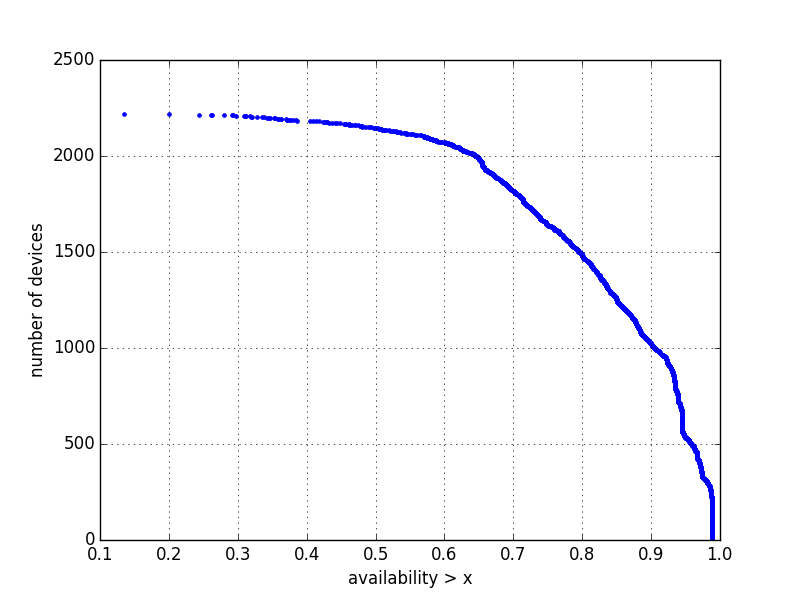
\includegraphics[width=\linewidth]{figures/250-test_dw-availability-CDF.png}
  \caption{Heartbeat by device}
  \label{fig:availability-device}
\end{subfigure}
%
\hspace{-1em}
%
\begin{subfigure}[b]{0.5\linewidth}
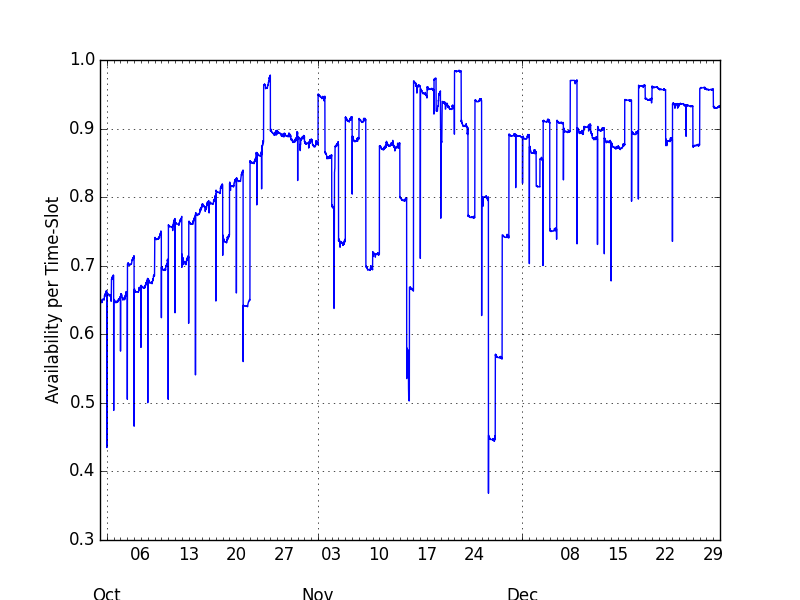
\includegraphics[width=\linewidth]{figures/250-test_dw-availability-by-date.png}
  \caption{Heartbeat by date}
  \label{fig:availability-date}
\end{subfigure}
%\hfill
%
\end{minipage}
\caption{Heartbeat, based on gateway device responsiveness. (Make common eps 
plot of heartbeat -- 8 control sets (half filtered) + test sets vs 
availability.) }
\label{fig:availability}
% created using docs/metadata-separated.log
\end{figure}


We sliced the sanitized \test set based on the date range of each 
individual \control set for comparison. We compared each of these tests 
individually to ensure that there are no outliers. We refer to the \test and 
\control sets in this case simply as datasets $set_1 - set_8$, where $set$ is 
\test or \control. We also sliced and combined the sanitized data to give us 
\control and \test data for each month, referred to as $set_{oct}$, $set_{nov}$, 
$set_{dec}$. Finally, we combine all \control sets to form a large concatenated 
dataset over the same date range as the complete \test dataset, and we refer to 
this simply as $set_{full}$. 

In the following analysis, we only present results for $set_{full}$, unless the 
behavior of an individual dataset varies significantly from the overall behavior 
and requires mention.

\subsection{Relevance of the Data}
\label{subsec:data-relevance}
\todo{REDO: not as limitations}

In this section we describe how the Comcast database collected is both granular 
as well as unbiased. This database enables us to study usage behavior in a 
controlled setting. Beside, because of following properties, it is legitimized 
our use of it to compare and validate the \FCC policy.

% why only byte counters are okay for this work
\paragraph{Study Byte Counters:} The purpose of this work is to study the usage 
characteristics, irrespective of the application responsible for such usage. 
%This is bolstered by FCC's decision of net neutrality 
Limiting ourselves to just byte counters makes our analysis easily extendible 
to any ISP, and the FCC, interested in doing a similar study at a larger 
scale, without the risk of leaking PII. A study of applications has already 
been performed extensively by Sandvine ~\cite{}, as well as other researchers.


\paragraph{Granularity of 15 minutes:} Broadband usage evaluated by commercial 
groups ~\cite{}, or governmental survey bodies, usually employed by the FCC, 
tends to focus on aggregated usage statistics over months, long term trends, and 
applications. In our work we specifically focus on data transferred in 15 
minutes, to avoid short term bursts that max out the capacity, but account for 
long term heavy flows (such as real time entertainment and voip calls) that will 
continuously max out the access link. This gives us a granularity fine grained 
enough to study major changes in usage characteristics (such as peak trends) 
while ignoring short term bursts of traffic (such as browsing)

Note that byte counter readings collected every 15 minutes from multiple 
households were synchronized for consistency in measurements.

\paragraph{High Tier Measurements:} We limit ourselves to analyzing usage 
patterns in the high capacity access link tier only. The \test dataset was 
collected by increasing the capacity from 105 Mbps to to 250 Mbps for 2200 
randomly selected users, without their knowledge. This served a two-fold purpose 
in avoiding biases that studies on usage and capacity suffer from: (a) 
\emph{Avoid behavioral change bias:} offering users with high capacity a further 
increase without their knowledge avoids the risk of behavioral changes that may 
occur when one purposefully buys a higher bandwidth connection; and (b) 
\emph{Avoid frustrated user bias:} users already have a high capacity that gets 
upgraded, instead of opting for an upgrade because their previous capacity was 
insufficient for their usage. Studying datasets with these biases will always 
show a positive correlation between usage and capacity, and by examining a 
single high capacity tier, we avoid this.


\paragraph{Single ISP, Same Location:} No bias between service plans, pricing 
model, and traffic treatment. Controlled setting. Paths + performance should be 
similar and unbiased by the ISP as data is from one city. Also avoids local 
behavioral biases (if any).
This gives us a highly controlled setting to study usage behaviors in an 
unbiased manner across a very large set of users (15k \control and 1500 \test 
households). Thus we believe that are conclusions will be representative of 
broadband behavior in a general American urban city. We expect the baseline 
behavior of all users to be similar, and in fact, interpret any differences 
between the \control and \test set behavior as aggregate changes that occurred 
due to the an increase in access link capacity.
